\section{Enjoyability and usefulness according to the interviews}

At the end of each user study a semi-structured interview was conducted with the participant. These interviews revealed widely diverging views towards the enjoyability and usefulness of force feedback with \glspl{dmi}. Some feedback modes polarized participants' opinions while others kept them relatively unanimous. Furthermore, participants came up with new force feedback modes for HapSynth, general improvements for the device, and potential target audiences.

\textit{Varying opinions on enjoyability and usefulness.} Participants provided diverse takes on enjoyability and usefulness of having force feedback on \glspl{dmi}. Several participants thought feeling the force feedback was simply fun, and many deemed force feedback useful, saying how it helped to assure the device is responding to user actions, gave one more sense to work with, and could be used to help guide the user towards a desired, possibly predefined, position, for example in a live situation. Accessibility benefits for people with disabilities or lack of perfect pitch was also brought up.

More reserved participants were worried about the limited usability of force feedback. They thought that the usable range between "not strong enough force feedback to have any benefit" to "too strong feedback it becomes irritating/hindering" would be quite small, and especially on stage situations the force feedback could easily be lost under the rumble of the shaky and noisy environment. Some participants were unable to tell whether force feedback brought more benefits or drawbacks.

In the negative end several participants thought force feedback either wasn't useful or actually lowered the enjoyability and usefulness of a \gls{dmi}. Participants said that the force feedback felt useless, especially in the current implementation where the opposing force is always constant, and for already musically skilled users. Furthermore, force feedback was described unpleasant and hindering, participants telling how it was not fun to use the device when it was fighting back, hurting the fingers, and how it felt like it didn't let the user move the slider to a position they wanted to move it to, thus obstructing the usage.

\textit{Position mode divided opinions.} \textit{Position} mode, which was used to compare force feedback modes to \glspl{dmi} without those, was seen both better and worse compared to the modes with force feedback. Some participants thought \textit{Position} mode was more pleasant to use after using modes with force feedback, and more useful as it didn't restrict movement at all. In contrary, some participants disliked \textit{Position} mode as it didn't provide any resistance and thus felt too "slippery".

\textit{Detents mode divided opinions.} Like \textit{Position}, \textit{Detents} mode also split the participants. Some thought it was fun to use, felt natural, and helped with the tasks since there was a limited discrete number of positions to choose from. On the contrary, others saw \textit{Detents} limiting as it prevented using values between two detents and thus not allowing to fine tune the value. The strength of \textit{Detents} mode's force feedback was also reported to be too strong, as the pressure it applies to the fingers rendered usage to what was described as "awful" and even "painful".

\textit{Texture mode felt good, but usefulness was indecisive.} \textit{Texture} mode was widely regarded as the most enjoyable feeling mode. Participants liked its smooth and natural feel, giving just enough feedback to assure the device is working, especially compared to usage without any force feedback. However, participants weren't as unanimous on whether having \textit{Texture} feedback was useful or not. The little resistance it gave was deemed helpful to find positions more gradually, but also made it feel like it was constantly "slightly off".

\textit{Friction mode was mostly disliked.} Most participants thought \textit{Friction} mode felt unpleasant and was hindering the usability, although few reported contrariwise. Like with \textit{Detents} mode the feedback was described as too strong. That made usage irritating, and painful, and giving the impression the user is doing something wrong, perhaps moving the slider to the wrong direction, thus hindering the usability. On the other hand, few participants liked the strong feedback and how it enabled to make small adjustments.

\textit{Elasticity and Oscillation modes were fun.} Even though the actual tasks did not use \textit{Elasticity} or \textit{Oscillation} modes, I still let participants to test them if they wanted to for additional feedback. Neither of these modes allow user to move the slider and leave it to that position, which some participants wished would have been possible. However, both modes were considered fun to use and potentially usable options for performing.

\textit{New force feedback modes and usability improvements were devised.} Participants came up with ideas for new feedback modes, and some general usability improvements for a \gls{dmi} with force feedback. Force feedback could be used to effectively guide the user towards a predetermined position, either by applying stronger feedback the further away the user is from that position, or the reverse, stronger feedback the closer user gets to the position. The feedback could also match the sound, either by replicating the generated audio wave or mimicking the feel of an existing instrument. Some variations for \textit{Detents} mode were suggested, such as applying the feedback in a sawtooth wave pattern. Furthermore, combining two or more existing modes was brought up, either by applying them at the same time, or by applying them for different ranges of the slider. Some usability improvements were brought up, for example it was suggested that the part which transmits the force feedback could be bigger, letting the user feel the feedback with larger surface area of their hand.

\textit{Thoughts on user groups.} According to the participants, force feedback on a \gls{dmi} would either be niche feature or something that would garner a wide audience. On one hand, force feedback could be used for learning purposes, being useful for users who are new to \glspl{dmi}, but on the other hand it was described as an enthusiast feature, only suitable for people with some special requirements. It was left unclear whether these two groups would be mutually exclusive or separate coexisting groups.

In conclusion, with these interviews alone nothing decisive can be said about the enjoyability or usefulness of a force feedback enabled \gls{dmi}. However, the positive comments do support the idea, and encourage for further research of the topic. \textit{Texture} mode seemed to rise above other modes in terms of enjoyability (including \textit{Position}), while usefulness (and possible hinderance) of \textit{Detents} mode was recognized.

\section{Enjoyability and usefulness according to \gls{nasa-tlx} measures}

One-way \gls{anova} tests were performed for all \gls{nasa-tlx} dimensions combined and for each dimension separately, comparing the effect of the different force feedback modes to the perceived load. \gls{anova} from the combined dimensions did not show statistical significance, $F(1.8, 25.7) = 3.1, p > 0.05$. Likewise \textit{mental demand}, \textit{temporal demand}, \textit{own performance}, \textit{effort}, and \textit{frustration} dimensions did not show statistical significance. Results of those are presented in Table \ref{tlx-anova}.

\begin{table}[h!]
	\centering
	\begin{tabular}{ |c|c| }
		\hline
		\thead{Dimension} & \thead{\gls{anova}} \\
		\hline
		Mental demand & $F(2.8, 38.8) = 0.2, p > 0.05$ \\
		\hline
		Physical demand & $F(2.1, 29.1) = 3.9, p < 0.05$ \\
		\hline
		Temporal demand & $F(2.4, 32.9) = 1.8, p > 0.05$ \\
		\hline
		Own performance & $F(2.7, 38.5) = 0.3, p > 0.05$ \\
		\hline
		Effort & $F(2.0, 27.5) = 2.5, p > 0.05$ \\
		\hline
		Frustration & $F(1.5, 21.7) = 1.7, p > 0.05$ \\
		\hline
	\end{tabular}
	\caption{\gls{anova} results of \gls{nasa-tlx} individual dimensions. Only \textit{physical demand} shows statistical significance.}
	\label{tlx-anova}
\end{table}

On the other hand, \gls{anova} test from \textit{physical demand} did show some statistical significance, with $F(2.1, 29.1) = 3.9, p < 0.05$. Pairwise comparisons were done to compare the effect of the force feedback modes to \textit{physical demand}, but none of the comparisons showed statistical significance. However, Figure \ref{tlx-physical-chart} hints that \textit{Detents} and \textit{Friction} modes would be physically more demanding than \textit{Position} and \textit{Texture} modes.

\begin{figure}[h!]
	\centering
	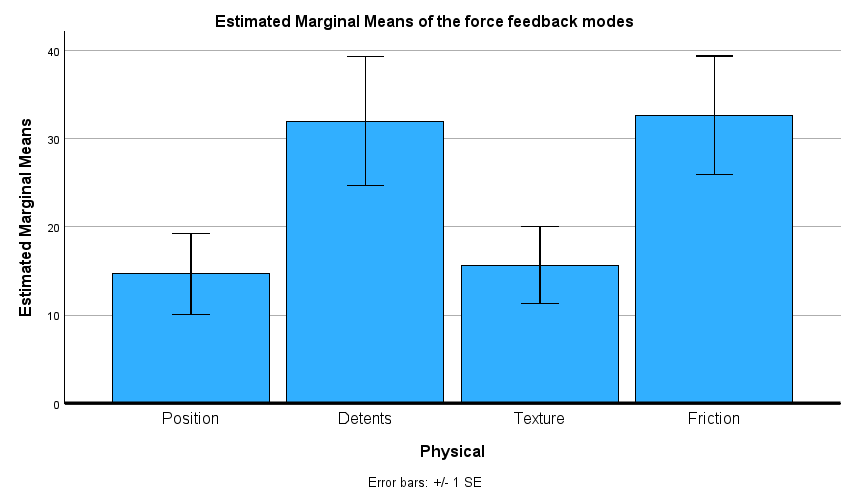
\includegraphics[width=1.0\linewidth]{figures/tlx-anova.png}
	\caption{Estimated Marginal Means of the force feedback modes to \textit{physical demand}.}
	\label{tlx-physical-chart}
\end{figure}

It can be extrapolated from these results that inclusion of force feedback in a \gls{dmi} does not significantly make its usage more or less demanding, excluding \textit{physical demand}, which might increase with some force feedback modes. Overall, with all \gls{nasa-tlx} dimensions, \textit{Texture} mode seemed to be slightly less demanding than \textit{Detents} and \textit{Friction} modes. These results seem to be in accordance with the interview results, \textit{Texture} mode being most liked possibly due to its lower demand, while \textit{Friction} mode's increase in especially \textit{physical demand} affecting the user experience in a negative way.

\section{Measured benefit}

Like for \gls{nasa-tlx}, one-way \gls{anova} tests were conducted for the measured time and accuracy data from the tasks, comparing the effect of the force feedback modes to time and accuracy, respectively. Results from neither of them showed any statistical significance, time being $F(2.7, 38.4) = 0.9, p > 0.05$ and accuracy $F(2.1, 29.3) = 0.9, p > 0.05$.

Based on these results there is no measurable benefit to time or accuracy from having force feedback in a \gls{dmi} in the context of the tasks of this user study. Like interviews and \gls{nasa-tlx} results, \textit{Friction} mode seemed to be slightly, albeit statistically insignificantly better than the other modes (including \textit{Position}). \textit{Detents} mode seemed to be the worst performing mode in both measures.